\documentclass{article}

% if you need to pass options to natbib, use, e.g.:
    \PassOptionsToPackage{numbers, compress}{natbib}
% before loading neurips_2020

% ready for submission
% \usepackage{neurips_2020}

% to compile a preprint version, e.g., for submission to arXiv, add add the
% [preprint] option:
    \usepackage[preprint]{neurips_2020}

% to compile a camera-ready version, add the [final] option, e.g.:
%     \usepackage[final]{neurips_2020}

% to avoid loading the natbib package, add option nonatbib:
    %  \usepackage[nonatbib]{neurips_2020}

\usepackage[utf8]{inputenc} % allow utf-8 input
\usepackage[T1]{fontenc}    % use 8-bit T1 fonts
\usepackage{hyperref}       % hyperlinks
\usepackage{url}            % simple URL typesetting
\usepackage{booktabs}       % professional-quality tables
\usepackage{amsfonts}       % blackboard math symbols
\usepackage{nicefrac}       % compact symbols for 1/2, etc.
\usepackage{microtype}      % microtypography
\usepackage{amsmath}
\usepackage{algorithm}
\usepackage{algpseudocode}
\usepackage{graphicx}
\usepackage{subfig}

\bibliographystyle{unsrtnat}

\title{Distributionally Robust Data Join for Image Classification}

% The \author macro works with any number of authors. There are two commands
% used to separate the names and addresses of multiple authors: \And and \AND.
%
% Using \And between authors leaves it to LaTeX to determine where to break the
% lines. Using \AND forces a line break at that point. So, if LaTeX puts 3 of 4
% authors names on the first line, and the last on the second line, try using
% \AND instead of \And before the third author name.

\author{%
  Anderson Lee \\
  Department of Computer Science \\
  University of Washington \\
  Seattle, WA 98195 \\
  \texttt{lee0618@cs.washington.edu} \\
  \And
  Rachel Hong \\
  Department of Computer Science \\
  University of Washington \\
  Seattle, WA 98195 \\
  \texttt{hongrach@cs.washington.edu} \\
}

\begin{document}

\maketitle

\begin{abstract}
  Distribution shift in image classification task has been a significant problem
  that compromises model's performance after deployment. Distributionally Robust
  Optimization (DRO) has been well-studied to train robust models for distribution shift by optimizing
  the worst case loss of a set of candidate distributions around an empirical
  distribution. In this paper, we study the adaptation of the method proposed 
  in \citep{awasthi2022distributionally} to incorporate unlabeled dataset with 
  auxiliary features to provide the set of candidate distributions to 
  optimize over, in the context of image classification tasks. We further 
  propose an alternative adversarial training approach which inherits the 
  motivation and is more tractable for deep neural network. In experiments on 
  CIFAR-100 and CIFAR-100C \citep{hendrycks2019robustness}, we are able to 
  observe some robustness when evaluated on severely corrupted images.
\end{abstract}

\section{Introduction}
Distribution shift is more than common in image classification task such as 
background changes in the wild for different camera traps, tumor identification
data from different hospitals, and autonomous driving decision-making 
when real-world scene changes. \citep{yao2022wild,malinin2021shifts} 
While deep neural network and vision transformer 
become more prevalent in high-stake classification tasks such as medical image scan 
and autonomous driving, ensuring the robustness of model on out-of-distribution 
inference is essential and requires different sets of training approaches 
than classical empirical risk minimization. Two main approaches to improve model's
robustness are Distributionally Robust Optimization and Adversarial Training.

Distributionally Robust Optimization (DRO) has been a well-studied approach 
to train a distributionally robust model by optimizing the worst case distribution
loss around the empirical distribution. \citep{rahimian2019distributionally} The set 
of distributions to be considered is often called \textit{ambiguity set}. A common 
phenomenon when solving distributionally robust optimization problem to train 
a predictor is that the predictor becomes overly-pessimistic and is not able 
to confidently predict any outcome. This phenomenon usually arises from having 
a too large ambiguity set that encompasses non-tractable worst case distribution.
The methods to determine the ambiguity set are therefore important in order 
to include the ideal wild distribution in the ambiguity set while not including 
to many unlikely distributions to optimize the model over. 

There have been multiple studies on how to define a good ambiguity set in both 
the definition of distance metrics that render the ambiguity set to be centered 
around the empirical distribution within some radius such as Prohorov metric
\citep{Erdogan2006AmbiguousCC} and Wasserstein metric \citep{esfahani2015data}.
Another set of methods to formulate ambiguity set is to utilize the moment of 
probability distributions such as \textit{Chebyshev ambiguity set}. 
\citep{rahimian2019distributionally}

In addition to choosing the definition of ambiguity set, another level beyond 
is to further articulate the ambiguity set for a certain classification task. 
\citep{sagawa2019distributionally} proposes a modified loss function 
to optimize extending from traditional DRO objective in favor of the emphasis 
on group information shift during inference time. \citep{awasthi2022distributionally}
takes advantages of unlabeled dataset with auxiliary features to define 
the ambiguity set with Wasserstein metric. Similarly, \citep{frogner2019incorporating}
incorporates unlabeled data to formulate the DRO objective to derive a 
tractable ambiguity set. 

Adversarial Training (AT) perturbs training data as a way to simulate distribution 
shift or even worse and unrealistic case. While AT perturbs 
each sample in different ways, DRO focuses on the entire distribution shift. 
AT can be viewed as shifting the empirical distribution to some point around 
itself depending on the actual implementation. In other words, in the perspective
of ambiguity set, it's a set with a singular point. \citep{Staib2017DistributionallyRD}
shows that a lower bound of AT loss on point-wise perturbation by the worst case 
distribution loss. In the context of image classification, \citep{carmon2019unlabeled}
incorporates unlabeled images to perform AT and shows improvement in both accuracy 
and robustness.

While unlabeled data is commonly believed to be much more accessible than 
labeled data, there have been only a few works on utilizing unlabeled 
data to improve both robustness and performance of the model. Beyond 
unlabeled data with the same set of features, auxiliary features in 
unlabeled data are also common such as in the context of medical data 
from different hospitals or wildlife images from different monitoring
institutions. Taking advantage of the auxiliary features or even 
multimodal features to train a joint distribution predictor or even 
one with performative marginal prediction with a subset of features
can be potential as a way to refine the ambiguity set.


In this work, we follow up the empirical work in the context of image 
classification task to take advantage of theoretical guarantees on 
the robustness in \citep{awasthi2022distributionally}. Besides, we also present an AT approach that intuitively
simulates the motivation with more randomness and less theoretical backbone
but with easier implementation and training stability.

\section{Problem Setup}
\subsection{Distributionally Robust Data Join (DRDJ)}
In \citep{awasthi2022distributionally}, two datasets $S_A$ and $S_P$ are 
given where $S_A$ is an unlabeled dataset with shared features $x$ and auxiliary features $a$ and 
$S_P$ is a labeled dataset with shared features $x$ and labels $y$. The 
respective empirical distributions of $S_A, S_P$ are denoted as 
$\tilde{\mathcal{P}}_{S_A}$ and $\tilde{\mathcal{P}}_{S_P}$. The 
ambiguity set defined is 
\begin{align*}
  W(S_A, S_P, r_A, r_P) = \{ \mathcal{Q} \in \mathbb{P}_{(\mathcal{X}, \mathcal{A}, \mathcal{Y})}  : \mathcal{D}_{d_A}(\mathcal{Q}_{\mathcal{X}, \mathcal{A}}, \tilde{\mathcal{P}}_{S_A}) \le r_A, \mathcal{D}_{d_P}(\mathcal{Q}_{\mathcal{X}, \mathcal{Y}}, \tilde{\mathcal{P}}_{S_P}) \le r_P\}
\end{align*}
where $\mathcal{D}_{d_A}$ is Wasserstein distance between marginalized $\mathcal{Q}_{\mathcal{X}, \mathcal{A}}$ and the empirical unlabeled distribution $\tilde{\mathcal{P}}_{S_A}$,
and $\mathcal{D}_{d_P}$ represents the counterparts in empirical labeled distribution. $r_A, r_P$ represent the radius 
of the Wasserstein distance ball around the empirical distribution $\tilde{\mathcal{P}}_{S_A}$ and $\tilde{\mathcal{P}}_{S_P}$
respectively. Intuitively, this ambiguity set represents the intersection between 
the Wesserstein ball around two empirical distributions with constant parameter radius 
$r_A, r_P$.  The objective of DRO following this ambiguity set is
\begin{align*}
  \min_{\theta \in \Theta} \sup_{\mathcal{Q} \in W(S_A, S_P, r_A, r_P)} \mathbb{E}_{(x, a, y) \in \mathcal{Q}} [\ell (\theta, (x, a, y))]
\end{align*}
where $\ell: \Theta \times (\mathcal{X} \times \mathcal{A} \times \mathcal{Y}) \to \mathbb{R}$ is the convex loss function, and 
$\theta$ is the model parameters. 
\subsection{Original Objectives}
\citep{awasthi2022distributionally} derives two 
objectives to optimize over simultaneously through a series of duality and problem reduction in 
the context of logistic regression.  
\begin{align*}
  &\Omega^A(\alpha_A, \alpha_P, \theta) 
  \\ &= \min_{\alpha_{A}\alpha_{P}\theta_{1}\theta_{2}}(\alpha_{A}r_{A}+\alpha_{P}r_{P})+\frac{1}{n_{A}n_{P}}\sum_{(i,j) \in M}(f(y_{j}^P\langle \theta , (x_j^P, a_i^A)\rangle)
  \\ & \qquad +\mathrm{max}(y_{j}^{P}\langle \theta, (x_j^P,a_{i}^{A}) \rangle -\alpha_{P}\kappa_{P},0)-\alpha_A||x_{i}^{A}-x_{j}^{P}||)
  \\ &\Omega^P(\alpha_A, \alpha_P, \theta) 
  \\ &= \min_{\alpha_{A}\alpha_{P}\theta_{1}\theta_{2}}(\alpha_{A}r_{A}+\alpha_{P}r_{P})+\frac{1}{n_{A}n_{P}}\sum_{(i,j) \in M}(f(y_{j}^P\langle \theta , (x_i^A, a_i^A)\rangle)
  \\ & \qquad +\mathrm{max}(y_{j}^{P}\langle \theta, (x_j^P,a_{i}^{A}) \rangle -\alpha_{P}\kappa_{P},0)-\alpha_P||x_{i}^{A}-x_{j}^{P}||)
\end{align*}
constrained by
\begin{align*}
  C^A &= \{(\alpha_A, \alpha_P, \theta) : ||\theta_1||_* \le \alpha_A + \alpha_P, ||\theta_2|| \le \kappa_A \alpha_A, \alpha_A < \alpha_P \}
  \\ C^P &= \{(\alpha_A, \alpha_P, \theta) : ||\theta_1||_* \le \alpha_A + \alpha_P, ||\theta_2|| \le \kappa_A \alpha_A, \alpha_A > \alpha_P \}
\end{align*}
for each objective respectively.

\textbf{Notations.} $x_i^A$ represents the $i$th sample from $S_A$, and $x_j^P$ represents the $j$th sample from $S_P$.
$M$ represents \textit{matching pairs}. $(i, j)$ exists in $M$ if and only if the shared features $x_i^A$ from $S_A$
is in the $k$-nearest neighbor of $x_j^P$ from $S_P$ or the other way around. $\alpha_A$ and $\alpha_P$ are 
trainable parameters resulting from duality of the original optimization problem. $\kappa_A$ and $\kappa_P$ 
are hyperparameters from duality of the original optimization problem as well. $\theta_1$ denotes the 
linear weights for shared features $x$ and $\theta_2$ denotes the linear weights for auxiliary features 
$a$. $\theta$ is the concatenation of $\theta_1$ and $\theta_2$.
The resulting $\theta$ will come from the minimum of these two objectives after optimizing. 
$f(t)$ represents logistic loss $\log (1 + \exp(t))$.

\section{Multi-class Vanilla DRDJ Objective Optimization}
\subsection{Image Classification Adaptation}
\textbf{Loss function}. We first replace the original logistic loss $f$ in the objective with cross entropy loss 
to support multiple classes

\textbf{Norm difference}. The norm term $||x_i^A - x_j^P||$ aims to present the similarity between 
two shared features in a matching pair. However, since image data has higher dimensionality and complexity,
direct comparison will not result in desirable property. We replace the norm term by the embeddings of 
images before final linear classifier layer $g(\theta, x_j^P, a_i^A)$. We use $g(\theta, x_j^P, a_i^A)$ 
to represent the trained model.

\textbf{Inner product}. The inner product $\langle \theta, (x_j^P, a_i^A) \rangle$ in $\Omega^A$ comes from 
vanilla logistic regression. In multi-class image classification task, we use predicted logits instead. From 
the previous notation, the predicted logits are denoted as $\text{Linear}(g(\theta, x_j^P, a_i^A))$ where 
the linear layer outputs number of classes according to the classification task.

\subsection{kNN Matching Pairs}
In the proposed algorithm from \citep{awasthi2022distributionally}, kNN is used 
for each sample in both $S_A$ and $S_P$ to generate the matching pairs $M$ as described above. However, 
for high dimensional data like images, it is significantly more difficult and less meaningful to 
naively do a similarity search on raw images using kNN algorithms. 

We first adopted SOTA masked autoencoder \citep{he2022masked} to find a lower dimensional representation 
of each image as their embeddings. Then, we perform similarity search on those embeddings as the 
source for generating matching pairs images. However, in our first batch of experiments, we were not 
able to generate good matching pairs based on qualitative analysis. For the time-constraint of 
this project, we simplify the matching pairs generation by using their ground truth labels even 
for the allegedly unlabeled dataset. The exact procedure is further specified in Section 5.1.

\subsection{Constraint Set}
In the original objective, the constraints $C^A$ and $C^P$ for $\Omega^A$ and $\Omega^P$ respectively 
are enforced by Projected Gradient Descent for optimization in the experiments in the 
original paper \citep{awasthi2022distributionally}. However, implementing Projected Gradient Descent
on GPU and PyTorch framework is quite difficult and doesn't have off-the-shelf supports from other 
packages. Therefore, we use penalty term to penalize solutions that violate the constraints sets. 
Specifically, there are three different penalty terms with different hyperparameter 
$\lambda_1, \lambda_2, \lambda_3$. 

In addition, since we are no longer in the realm of classical logistic regression, 
we cannot provide upper-bound on all parameters. Therefore, to simplify the problem, 
we only penalize on the weight parameters of the final classifier layer.
\begin{align*}
  \text{Penalty}^A &= \lambda_1 \cdot (||\theta_1||_* - (\alpha_A + \alpha_P)) + \lambda_2 \cdot 
  (||\theta_2|| - \kappa_A \alpha_A) + \lambda_3 \cdot (\alpha_A - \alpha_P)
  \\ \text{Penalty}^P &= \lambda_1 \cdot (||\theta_1||_* - (\alpha_A + \alpha_P)) + \lambda_2 \cdot 
  (||\theta_2|| - \kappa_A \alpha_A) + \lambda_3 \cdot (\alpha_P - \alpha_A)
\end{align*}


\subsection{Vanilla DRDJ Objective}
With the above adaptations and simplifications, the objective to optimize over becomes
\begin{align*}
  &\Omega^A(\alpha_A, \alpha_P, \theta) 
  \\ &= \min_{\alpha_{A}\alpha_{P}\theta_{1}\theta_{2}}(\alpha_{A}r_{A}+\alpha_{P}r_{P})+\frac{1}{n_{A}n_{P}}\sum_{(i,j) \in M}(\text{CrossEntropyLoss}(\text{Linear}(g(\theta, x_j^P, a_i^A)), y_j^P)
  \\ & \qquad +\mathrm{max}(\text{Linear}(g(\theta, x_j^P, a_i^A))_{y_j} -\alpha_{P}\kappa_{P},0)-\alpha_A||g(\theta, x_{i}^A) - g(\theta, x_{j}^P)||)
  \\ &\Omega^P(\alpha_A, \alpha_P, \theta) 
  \\ &= \min_{\alpha_{A}\alpha_{P}\theta_{1}\theta_{2}}(\alpha_{A}r_{A}+\alpha_{P}r_{P})+\frac{1}{n_{A}n_{P}}\sum_{(i,j) \in M}(\text{CrossEntropyLoss}(\text{Linear}(g(\theta, x_i^A, a_i^A)), y_j^P)
  \\ & \qquad +\mathrm{max}(\text{Linear}(g(\theta, x_j^P, a_i^A))_{y_j} -\alpha_{P}\kappa_{P},0)-\alpha_P||g(\theta, x_{i}^A) - g(\theta, x_{j}^P)||)
\end{align*}


\section{Distributionally Robust Adversarial Attack}
\subsection{Intuition}
The motivation of data join for distributionally robust optimization is to take advantage of 
an anchor distribution (the unlabeled dataset) and to believe that training the model by 
optimizing the worst case loss in the set of distributions within the intersection of 
the Wasserstein balls around two empirical distributions will lead to a more robust 
model. Instead of optimizing the objective that is intrinsically difficult because of 
the theoretical constraints, it might be more desirable and easier to implement perturbation
as adversarial attack that simulates the motivation.

Figure \ref{fig:wasserstein_ball} shows the intuition of optimizing over the intersection ambiguity set 
in original DRDJ. We can simulate the set of distributions by leveraging original samples from 
two empirical distributions and perturbed samples. \citep{Staib2017DistributionallyRD}
uses point-wise adversarial training as an alternative of traditional DRO objective 
where ambiguity set is defined as a Wasserstein ball around a single empirical distribution. 
In our case, since we are interested in an intersected set of distributions, a doubly 
constrained adversarial perturbation is still less feasible. Instead, we perform separate
perturbations on the two samples we have, $x_i^A, x_j^P$ in a matching pair defined 
the same way as vanilla DRDJ.

\begin{figure}
  \centering
  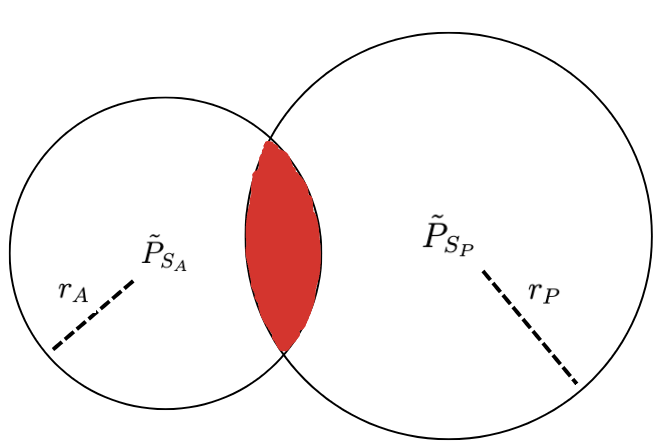
\includegraphics[width=7cm]{plots/wasserstein_ball.png}
  \caption{Wasserstein Ball Ambiguity Set}%
  \label{fig:wasserstein_ball}%
\end{figure}

\subsection{Perturbation}
We define $\tilde{x}_i^A$ as the perturbed sample of $x_i^A$ and $\tilde{x}_j^P$ as the perturbed 
sample of $x_j^P$. They are formally defined as 
\begin{align*}
  \tilde{x}_i^A &= \text{arg} \max_{x \in \mathcal{B}(x_i^A, r_A)} ||\text{Linear}(g(\theta, x, a_i^A)) - 
  \text{Linear}(g(\theta, x_j^P, a_i^A))||_2
  \\ \tilde{x}_j^P &= \text{arg} \max_{x \in \mathcal{B}(x_j^P, r_P)} ||\text{Linear}(g(\theta, x_i^A, a_i^A)) - 
  \text{Linear}(g(\theta, x, a_i^A))||_2
\end{align*}
where $x_i^A, x_j^P$ inherit the notations from above in a matching pair,
$\mathcal{B}(x_i^A, r_A)$ denotes a L2-norm ball with radius $r_A$ around $x_i^A$, 
and $\mathcal{B}(x_j^P, r_P)$ denotes a L2-norm ball with radius $r_P$ around $x_j^P$.

These two perturbed samples can be viewed as the samples close to the original sample ($x^A_i$ or $x^P_j$)
within some radius in a L2-norm ball that make their predicted logits the \textbf{most different} 
from the \textit{anchor sample} which is the other original sample that is not being perturbed (e.g. $x^A_i$ is the anchor if perturbing $x^P_j$). 
The perturbed samples are not at all guaranteed to be located in the intersected set because 
there exists no constraint on the radius with the other ball. In fact, it's more likely that they are located on 
the opposite direction of the other anchor sample because the optimization problem 
maximizes the difference of predicted logits between them. We believe that optimizing 
over both of them with some hyperparameter weights at the same time will be sufficient to 
perform well on the intersected set of interest because a well-trained predictor should 
balance the performance well on samples extremely far from $\tilde{P}_{S_A}$ and close 
to $\tilde{P}_{S_P}$ or the other way around.

\subsection{Loss Function}
With perturbed samples, we can weigh the Cross-entropy loss of original samples and 
adversarial samples in training time to emphasize the focus on perturbed samples 
or empirical distribution. The motivation to weigh in the empirical loss instead of 
only the perturbed sample loss is to guide the model to learn the classification 
task in earlier training time as the perturbation depends on the model's ability 
to differentiate predicted logits from different types of images. In other words,
the perturbation task requires the model's predictive power in order to be 
significantly meaningful. Thus, the loss function can be formally defined as
\begin{align*}
  L_{\text{adversarial}} &= w_1 \cdot \ell(\theta, (x_j^p, y_j^p)) + w_2 \cdot \ell(\theta, (\tilde{x}_j^p, y_j^p))
    + w_3 \cdot \ell(\theta, (x_i^a, y_j^p)) + w_4 \cdot \ell(\theta, (\tilde{x}_i^a, y_j^p))
\end{align*}

\subsection{Training Schedule}
\begin{algorithm}
  \caption{Adversarial DRDJ Train One Epoch}
  \begin{algorithmic}[1]
    \For{$X_i^A, A_i^A, X_j^P, Y_j^P$ in batch}
      \State $\tilde{X}_i^A, \tilde{X}_j^P \gets \text{Solve argmax problem}$
      \State Calculate loss function $L_{\text{adversarial}}$
      \State Backward Propagation as usual
    \EndFor
  \end{algorithmic}
\end{algorithm}

\section{Experiments}
\subsection{Setup}
Due to time constraints, the main experiments were done in CIFAR-100 image dataset. 
Instead of trying to work with two datasets with one labeled and the other 
unlabeled and equipped with auxiliary features, we simplify the problem to focus 
on \textbf{splitting CIFAR-100 to two subsets} and \textbf{limit ourselves to no 
auxiliary features for images} for time being. 

CIFAR-100 contains 60,000 images with 600 images per class. We divide 100 into validation 
set per class and 250 into each subset group denoted as $S_A$ and $S_P$. Ideally, we should 
not take advantage of labels from $S_A$ at all cost. However, due to the forementioned 
challenge in autoencoder similarity search, we use $S_A$'s labels to generate matching pairs 
by randomly sample 1000 pairs of images for each class, which results in a total number of 
100,000 matching pairs.

CIFAR-100C \citep{hendrycks2019robustness} consists of CIFAR-100 dataset's images 
corrupted in 19 different contexts including Gaussian Blurring, snowing effects, and 
other background changes simulation in two severity level. We'll use \textit{easy 
corruption} and \textit{hard corruption} to indicate these two severity levels of 
corruption. The accuracy is calculated by averaging the accuracies in all 19 contexts
of corruptions.

We use ResNet50 as the baseline model and backbone model for both Vanilla DRDJ and 
Adversarial DRDJ approaches. It is worth noted that the baseline is only trained on 
$S_P$ which only consists of less than half of images from CIFAR-100 because 
we assume the labels are not accessible from $S_A$. 

\subsection{Metrics}
Concluded from \citep{taori2020measuring}, accuracy doesn't imply robustness. One must 
evaluate the robustness of the model based on its relative performance (accuracy) 
to the baseline. We adopted a similar evaluation plot with regular test accuracy 
on the x-axis and corrupted test accuracy on the y-axis. An ideally perfect 
robust model should have accuracy aligned with the line $y = x$, which indicates 
no drop in corrupted accuracy compared to its regular test counterpart. We also 
plot the linear fit of all baseline models, which in our case is a series of 
ResNet50 in different configurations. A robust model should be positioned above 
the linear fit because it is expected to achieve better corrupted test accuracy 
than its similar-performance counterparts.

\subsection{Vanilla DRDJ}
Figure \ref{fig:vanilla_DRDJ_evaluation} shows constantly low performance of Vanilla DRDJ models. 
There is no obvious robustness in either easy or hard corruption. There are a number of 
potential failure reasons:

\textbf{Relaxed Constraint Set}. Previously, we use penalty term to avoid using Projected 
Gradient Descent that enforces the constraint set to hold. This might intrinsically break 
the theoretical guarantees and lead to a worse solution that becomes more and more pessimistic
in prediction. During training, we observe that $\alpha_A$ and $\alpha_P$ usually don't 
follow the constraints they are meant to be within even with the penalty terms.

\textbf{Weak Distribution Shift}. In our experiments, we divide the same dataset CIFAR-100
into two groups. While there might exist some distribution shift in these two subsets, but 
they are minimal. The fact that $\tilde{P}_{S_A}$ and $\tilde{P}_{S_P}$ are much closer 
might sacrifice the accuracy for unrealistic robustness in some random
worst case distribution.

\textbf{Adaptation}. Previously, we change the norm term and other terms in the objective 
to adjust to Multi-class image classification setting with neural networks. However, 
these simplifications are not supported by theoretical guarantees and might require 
more investigation than simply changing it to a desirable form at no cost.

\begin{figure}
  \centering
    \subfloat[\centering Vanilla DRDJ on Easy Corruption]{{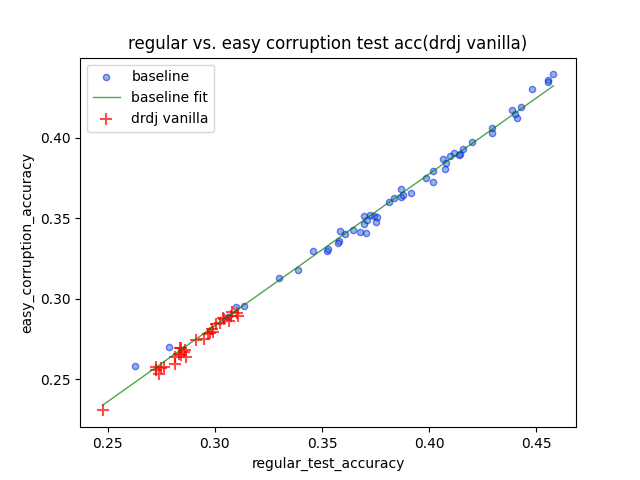
\includegraphics[width=7cm]{plots/reg_easy_acc_vanilla.png} }}%
    \qquad
    \subfloat[\centering Vanilla DRDJ on Hard Corruption]{{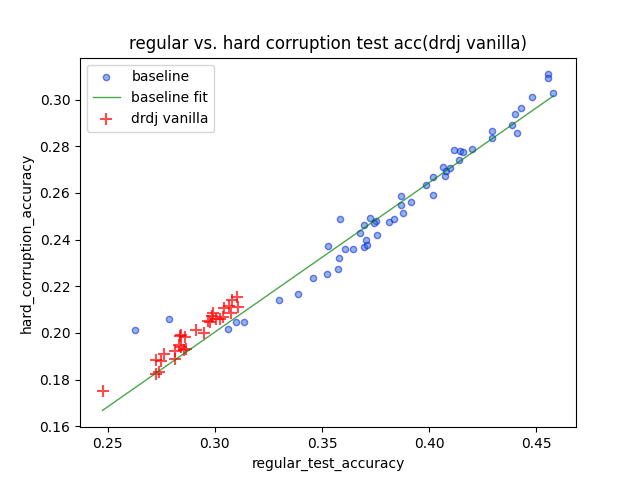
\includegraphics[width=7cm]{plots/reg_hard_acc_vanilla.png} }}%
    \caption{Vanilla DRDJ Evaluation on CIFAR-100C}%
    \label{fig:vanilla_DRDJ_evaluation}%
\end{figure}

\subsection{Adversarial DRDJ}
Figure \ref{fig:adversarial_DRDJ_evaluation} shows that under easy corruption, AT doesn't lead 
to a consistently robust model compared to the baseline. However, with harder corruption, 
we can see all the Adversarial DRDJ trained models have higher robustness because they 
are all positioned above the linear fit of the baseline. We also see that there is no 
overall lower trend in performance (regular test accuracy). This tells us that the AT 
DRDJ training approach is more tractable and easier to make the model learn the right 
solution.

\textbf{Weak Distribution Shift}. While the intuition set up previously 
is favorable, the simplifications done to split a dataset into two doesn't provide 
much meaningful distributions shift for our adversarial attack to be meaningful. 
The variance in adversarial attack will likely to override its intended effects 
when the corruption is not severe. 

\begin{figure}
  \centering
    \subfloat[\centering Adversarial DRDJ on Easy Corruption]{{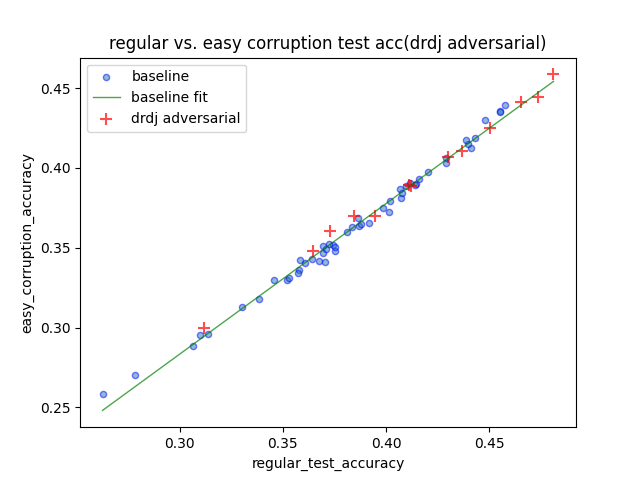
\includegraphics[width=7cm]{plots/reg_easy_acc_adversarial.png} }}%
    \qquad
    \subfloat[\centering Adversarial DRDJ on Hard Corruption]{{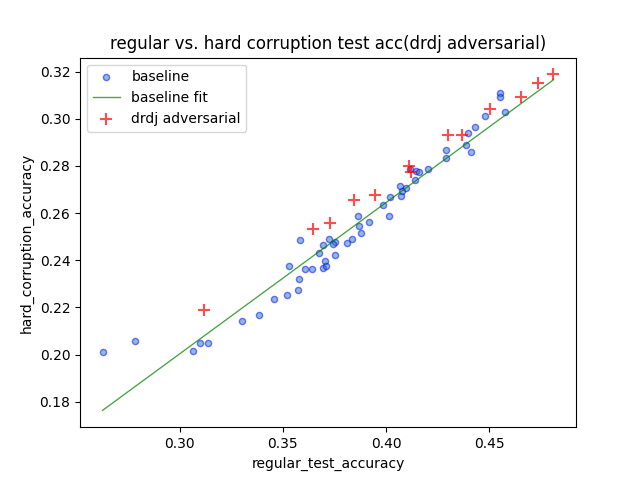
\includegraphics[width=7cm]{plots/reg_hard_acc_adversarial.png} }}%
    \caption{Adversarial DRDJ Evaluation on CIFAR-100C}%
    \label{fig:adversarial_DRDJ_evaluation}%
\end{figure}


\section{Future Direction}
\subsection{Revert Simplifications}
\textbf{Generating matching pairs with kNN}.
The matching pairs generation is simplified in this work due to time-constraints.
Image data similarity search is primitively more difficult and time-consuming
because of its high dimensional features. We aim to revisit autoencoder 
approach but also think of other alternatives since the pipeline involving 
training an antoencoder could be less tractable.


\textbf{Incorporate auxiliary features}. In this work, we didn't utilize any auxiliary features. We specify future 
directions for auxiliary features in Section 6.2. 

\textbf{Utilize unlabeled data from a natively different dataset}. In our experiments, we split CIFAR-100 to two subsets and ignore the second 
subset's labels. However, such practice is not reflective of the target 
scenario this work is aiming at. Therefore, simulating the scenario with 
a dataset that (1) shares some features with the labeled set, 
(2) is unlabeled, and (3) provides larger amount of data, will be the 
ideal candidate for our next batch of experiments.


\subsection{Auxiliary Features}
For simplicity, we didn't explore auxiliary features in this work even 
though the proposed training approach is natively adaptive to auxiliary 
features. Additional features like metadata have promising potentials as explored 
by \citep{mcauley2012image}. In addition, multimodal classification task can 
also be integrated into our proposed framework with some modifications as 
large video dataset with audio modality provides a lot of richness but 
requires tremendous labeling efforts. We aim to continue investigating 
more empirical results for multimodal tasks including audiovisual, text-visual,
and other tabular metadata information.

\subsection{Fairness}
While the model's robustness is critical and the goal of this work, 
we believe this work also has potential impact on group fairness. Group 
information can be treated as auxiliary features in our work. Although 
the dataset with group information is unlabeled, our work allows incorporating 
group information in training an image classification model in tasks like 
facial recognition and provides more fair predictor than one trained purely 
on unbalanced and biased dataset with labels.

\newpage
\bibliography{reference}
\end{document}